% !TeX spellcheck = it_IT
\section{Complessità}

\subsection{Notazione asintotica}
Quando scriviamo un algoritmo, per calcolarne il costo, bisogna fare una serie di assunzioni sulla macchina astratta su cui lavoriamo:
\begin{itemize}
	\item L'accesso alle celle di memoria avviene in tempo costante.
	\item Le operazioni elementari avvengono in tempo costante:
	\begin{itemize}
		\item Operazioni aritmetiche e logiche della ALU
		\item Gli assegnamenti
		\item I controlli del flusso (salti, assegnamento al registro PC)
	\end{itemize}
	
\end{itemize}
Per calcolare il costo degli algoritmi si possono utilizzare due modelli:
\begin{enumerate}
	\item \textbf{Word model}: tutti i dati occupano solo una cella di memoria.
	\item \textbf{Bit model}: unità elementare di memoria \emph{bit}, si usa quando le grandezze sono troppo grandi.
\end{enumerate}

\noindent Esistono una serie di parametri da \textbf{analizzare} quando scriviamo una algoritmo. Essi permettono di garantire il suo corretto funzionamento e la sua ottimizzazione. Sono i seguenti:
\begin{itemize}
	\item \textbf{Complessità}: ovvero l'analisi dell'utilizzo delle risorse: 
	\begin{itemize}
		\item tempo di esecuzione
		\item spazio di memoria per i dati in ingresso e in uscita. Viene rappresentato astrattamente dal numero di celle di memoria (word model)
		\item banda di comunicazione (per esempio nel caso il calcolo sia distribuito)
	\end{itemize}
	Non sarà quasi mai possibile avere un programma che è sia efficiente in termini di tempo che in di spazio (\emph{coperta corta}).
	\item \textbf{Correttezza}: Indica se l'algoritmo fa quello per cui è stato progettato. Si esegue in due modi:
	\begin{itemize}
		\item \underline{dimostrazione formale} la quale permette di dimostrare la correttezza risolvendo tutte le istanze del problema
		\item \underline{ispezione formale} nella quale si usano metodi come il \textbf{testing} o il \textbf{profiling}. Il primo prevede di provare il programma nelle situazioni critiche, il secondo analizza il tempo che la CPU impiega per elaborare una determinata parte del programma.
	\end{itemize}
	\item \textbf{Semplicità}: Indica se l'algoritmo è facile da capire e manutenere. Un algoritmo è semplice quando usa identificatori significativi, quando è ben commentato, se usa strutture dati adeguate e se rispetta gli standard.
\end{itemize}

\begin{definition}[Complessità di un problema]
	La complessità di un problema $P$ è la complessità del miglior algoritmo $A$ che lo risolve.
\end{definition}
Per trovare la complessità del problema partiamo dal fatto che, dato un algoritmo $A$, la complessità di $A$ determina un limite superiore alla complessità di $P$ (cioè quando si verifica il caso peggiore uso $A$ per risolvere $P$).\\
Se riusciamo a determinare un limite inferiore $g(n)$ per $P$, per ogni algoritmo $A$ che risolve $P$ ho che $A \in \Omega(g(n))$, dove $g(n)$ è il minimo numero di operazione che posso impiegare per risolvere $P$. Quindi possiamo dire che:
\begin{equation}
	A \in \Theta(g(n)) \Longrightarrow A \text{ ottimo} \footnote{Ricorda che dire che $A \in \Theta(g(n))$ vuol dire che $A \in O(g(n))$ e $A \in \Omega(g(n))$}
\end{equation}
Per fare ciò bisogna anche andare a calcolare il limite inferiore del caso pessimo, e ciò è possibile tramite 3 metodi: la \textbf{dimensione dei dati}, gli \textbf{eventi contabili} e gli \textbf{alberi decisionali}.

\begin{itemize}
	\item \textbf{Dimensione dei dati}: Se la soluzione di un problema richiede l'esame di tutti i dati in input, allora $\Omega(n)$ è un limite inferiore. \emph{E.g. sommare tutti gli elementi di un array.}
	\item \textbf{Eventi contabili}: se la soluzione di un problema richiede la ripetizione di un certo evento, allora il numero di volte che l'evento si ripete (moltiplicato per il suo costo) è un limite inferiore.
	\item \textbf{Alberi di decisione}: sono alberi in cui
	\begin{itemize}
		\item ogni nodo non foglia effettua un test su un attributo
		\item ogni arco uscente da un nodo è un possibile valore dell'attributo
		\item ogni nodo foglia assegna una classificazione
	\end{itemize}
	Si applica a problemi risolubili attraverso sequenze di decisioni che via via riducono lo spazio delle soluzioni.
	\begin{figure}[!h]
		\centering
		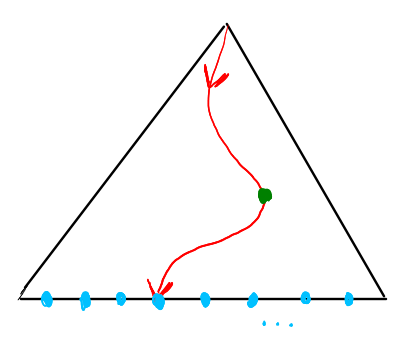
\includegraphics[width=5cm]{images/albero-decisionale.png}
		\caption{Albero decisionale}
	\end{figure}
	\\In figura vediamo che dalla situazione iniziale, tramite un \color{red} percorso radice-foglia \color{black} (ovvero un'esecuzione dell'algoritmo), otteniamo una tra le possibili \color{blue} soluzioni \color{black}  (foglie) passando per diverse \color{green} decisioni \color{black} (nodi interni).
	\begin{note}
		Alcune formule importanti per gli alberi:
		\begin{itemize}
			\item  \textbf{Foglie}: $n^d$
			\item \textbf{Profondità} $d \leq \log_n$ foglie (è esattamente uguale solo se l'albero è completo)
			\item \textbf{Nodi}: $n^{d+1}-1$			
		\end{itemize}
	\end{note}
	\begin{example} Ricerca binaria di un elemento $k$ in un array $A$ di $n$ elementi. Ogni confronto tra $k$ e $A[cen]$ può generare 3 possibili risposte:
		\begin{itemize}
			\item $k < A[cen]$ ramo sinistro
			\item $k == A[cen]$ ramo centrale
			\item $k > A[cen]$ ramo destro
		\end{itemize}
	Abbiamo quindi che ogni confronto apre 3 possibili vie e dopo $i$ confronti avremo $3^i$ vie. Le possibili soluzioni sono $n+1$ ($k$ può essere in ognuna delle $n$ posizioni o non esserci). Avremo quindi:
	\begin{equation}
		3^i \geq n+1 > n \implies \text{binSearch} \in \Omega(\log_n)
	\end{equation}
		
	\end{example}
\end{itemize}

\subsection{Big-O notation}
La notazione Big-O ha molteplici scopi nella scrittura di un algoritmo.
\begin{itemize}
	\item Serve a rappresentare la complessità relativa di un algoritmo.
	\item Descrive le prestazioni di un algoritmo e come queste scalano al cresce dei dati in input.
	\item Descrive un limite superiore al tasso di crescita di una funzione ed è il caso peggiore.
\end{itemize}

\subsubsection{Limite superiore asintotico}
\begin{definition}[Limite superiore asintotico]
	Il limite superiore asintotico \footnote{\emph{Asintotico} indica che la definizione deve essere valida solo da un certo punto in poi scelto arbitrariamente.} si definisce come:
	\begin{equation}
		O(g(n)) = \{f(n) \mid \exists c, n_0 > 0 . \forall n > n_0, 0 \leq f(n) \leq c \cdot g(n)\}
	\end{equation}
\end{definition}
\noindent Si scrive come $f(n) \in O(g(n))$ oppure $f(n) = O(g(n))$ e si legge $f(n)$ è nell'ordine $O$ grande di $g(n)$.
\begin{example}
	Esempio di calcolo del limite superiore asintotico
\end{example}
\begin{wrapfigure}[7]{l}{8cm}
	\vspace{-15pt}
	\centering
	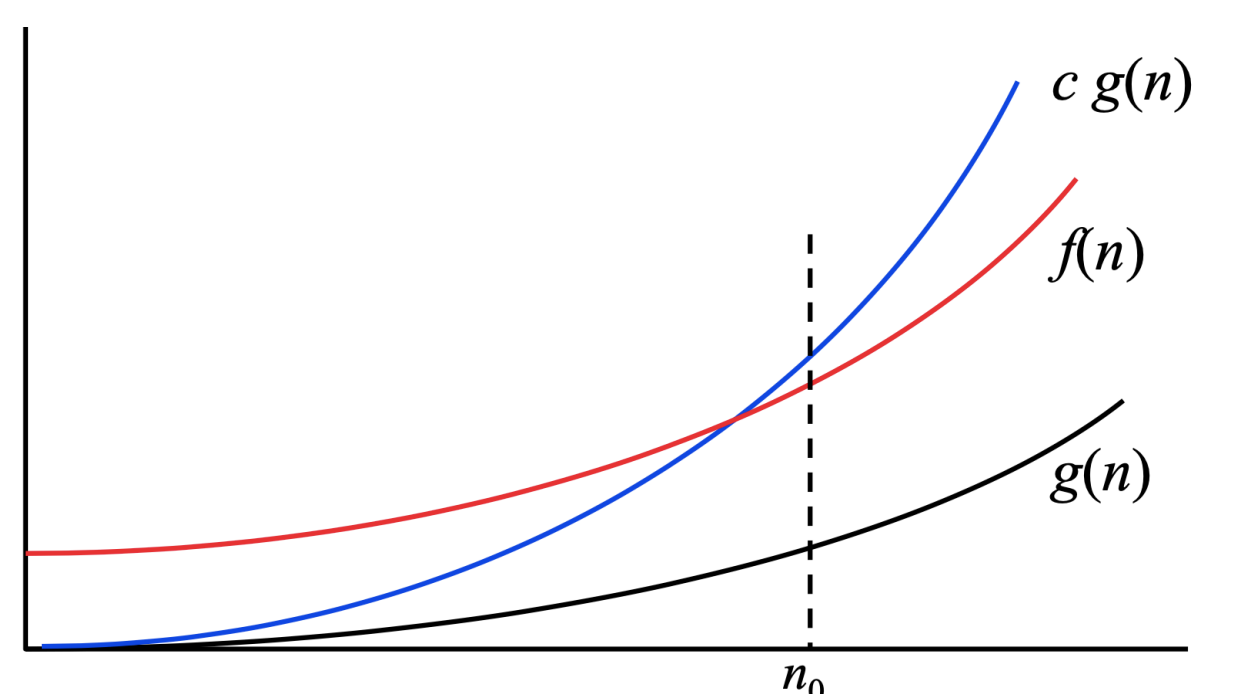
\includegraphics[width=6cm]{images/limite-superiore-asintotico.png}
	\vspace{-5pt}
	\caption{Limite superiore asintotico}
\end{wrapfigure}
Prendiamo due funzioni e determiniamo i punti $n_0$ e $c$ per cui è soddisfatta la definizione.
\begin{center}
	\vspace{-5pt}
	$f(n) = 3n^2 + 5$\hspace{30pt}$g(x)=n^2$
\end{center}
Stabiliamo un $c = 4$ e $n_0 = 3$.
\begin{enumerate}
	\item $4 \cdot g(n) = 4n^2 = 3n^2 + n^2 $
	\item $3n^2 + n^2 \geq 3n^2 + 9 $ (per ogni $n \geq 3$)
	\item $3n^2 + 9 > 3n^2+5 \Longrightarrow 4 \cdot g(n) > f(n)$
\end{enumerate}

\begin{note}
	Abbiamo disegnato solo il primo quadrante perché sia i dati in input che le operazioni da eseguire saranno sempre in numero positivo.
\end{note}

\subsubsection{Limite inferiore asintotico}
\begin{definition}[Limite inferiore asintotico]
	Il limite inferiore asintotico si definisce come:
	\begin{equation}
		\Omega(g(n)) = \{f(n) \mid \exists c, n_0 > 0 . \forall n > n_0, 0 \leq c \cdot g(n) \leq f(n) \}
	\end{equation}
\end{definition}
\noindent Si scrive come $f(n) \in \Omega(g(n))$ oppure $f(n) = \Omega(g(n))$ e si legge $f(n)$ è nell'ordine $\Omega$ grande di $g(n)$. Indica che quell'algoritmo non potrà mai fare di meglio.
\begin{example}
	Esempio di calcolo del limite inferiore asintotico. Prendiamo due funzioni e determiniamo i punti $n_0$ e $c$ per cui è soddisfatta la definizione.
\end{example}
\begin{wrapfigure}[6]{r}{8cm}
	\vspace{-15pt}
	\centering
	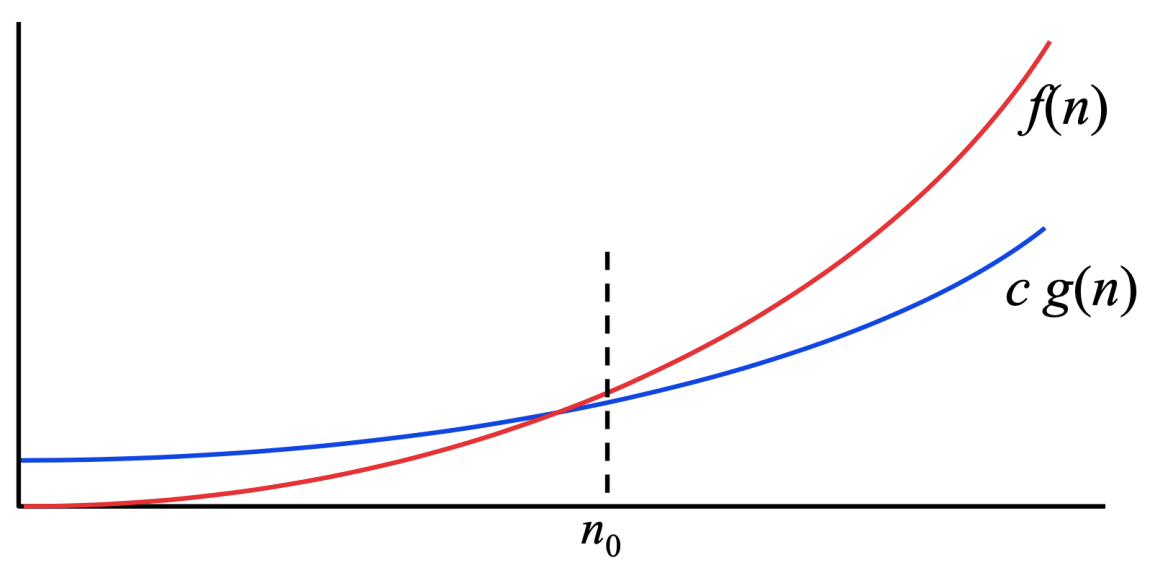
\includegraphics[width=6cm]{images/limite-inferiore-asintotico.png}
	\vspace{-5pt}
	\caption{Limite superiore asintotico}
\end{wrapfigure}

$f(n) = \frac{n^2}{2}-7$ \: \: \: $g(x)=n^2$\\
Stabiliamo un $c = \frac{1}{4}$ e $n_0 = 6$.
\begin{enumerate}
	\item $\frac{1}{4} \cdot g(n) = \frac{n^2}{4} = \frac{n^2}{2} - \frac{n^2}{4}$
	\item $\frac{n^2}{2} - \frac{n^2}{4} \leq \frac{n^2}{2} - 9 $ (per ogni $n \geq 6$)
	\item $\frac{n^2}{2} - 9 > \frac{n^2}{2}-7 \Longrightarrow \frac{1}{4} \cdot g(n) < f(n)$
\end{enumerate}

\subsubsection{Limite asintotico stretto}
\begin{definition}[Limite asintotico stretto]
	Il limite asintotico stretto si definisce come:
	\begin{equation}
		\Theta(g(n)) = \{f(n) \mid \exists c_1, c_2, n_0 > 0 . \forall n > n_0, 0 \leq c_1 \cdot g(n) \leq f(n) \leq c_2 \cdot g(n) \}
	\end{equation}
\end{definition}
\begin{wrapfigure}[5]{l}{8cm}
	\vspace{-10pt}
	\centering
	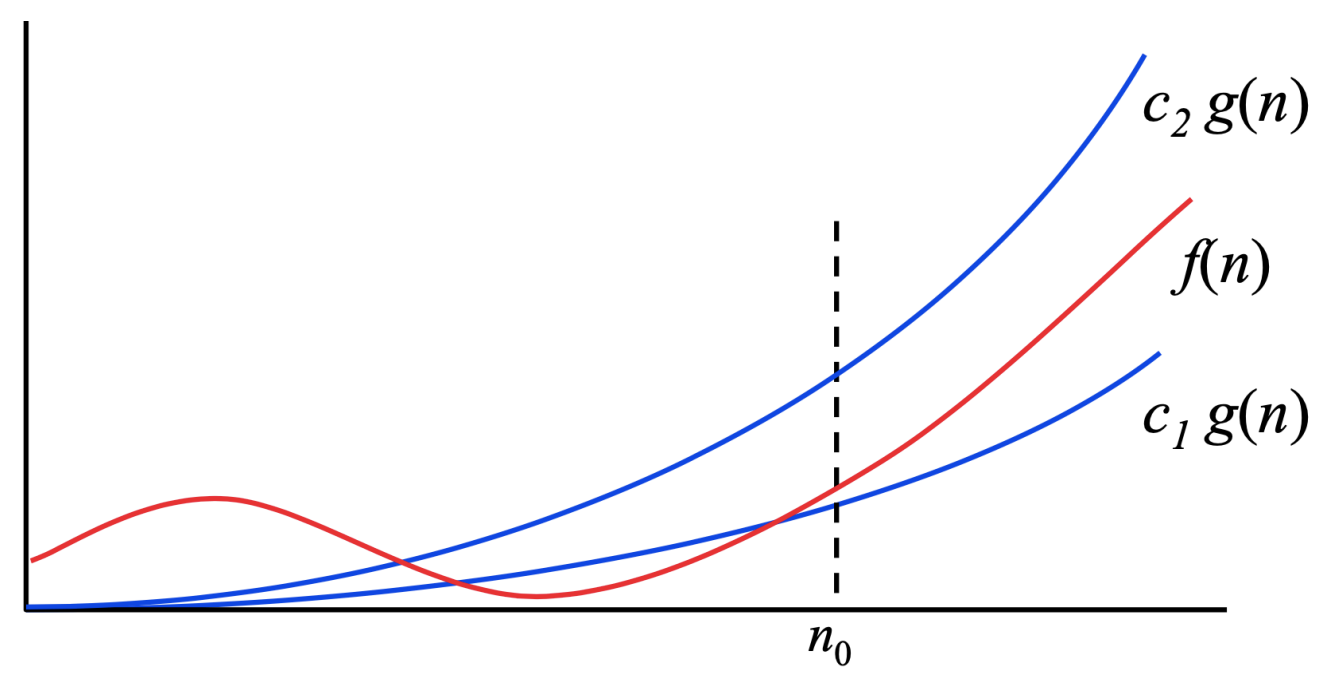
\includegraphics[width=6cm]{images/limite-asintotico-stretto.png}
	\vspace{-5pt}
	\caption{Limite asintotico stretto}
\end{wrapfigure}
Si scrive come $f(n) \in \Theta(g(n))$ oppure $f(n) = \Theta(g(n))$ e si legge $f(n)$ è nell'ordine $\Theta$ grande di $g(n)$.\\\\

\vspace{55pt}
Dalla definizione deriva che:
\begin{equation}
	f(n) \in \Theta(g(n)) \Longleftrightarrow f(n) \in \Omega(g(n)) \land f(n) \in O(g(n))
\end{equation}

\subsubsection{Teoremi sulla notazione asintotica}
\begin{theorem}
	Per ogni $f(n)$ e $g(n)$ vale che:
	\begin{enumerate}
		\item $f(n) = O(g(n)) \Longleftrightarrow g(n) = \Omega(f(n))$
		\item Se $f_1(n) = O(f_2(n)) \land f_2(n) = O(f_3(n)) \Longrightarrow f_1(n) = O(f_3(n))$
		\item Se $f_1(n) = \Omega(f_2(n)) \land f_2(n) = \Omega(f_3(n)) \Longrightarrow f_1(n) = \Omega(f_3(n))$
		\item Se $f_1(n) = \Theta(f_2(n)) \land f_2(n) = \Theta(f_3(n)) \Longrightarrow f_1(n) = \Theta(f_3(n))$
		\item Se $f_1(n) = O(g_1(n)) \land f_2(n) = O(g_2(n)) \Longrightarrow O(f_1(n) + f_2(n)) = O(max\{g_1(n),g_2(n)\})$
		\item Se $f(n)$ è un polinomio di grado $d \Longrightarrow f(n) = \Theta(n^d)$
	\end{enumerate}
\end{theorem}

\subsubsection{Limite superiore asintotico non stretto}
\begin{definition}[Limite superiore asintotico non stretto]
	Il limite superiore asintotico non stretto si definisce come:
	\begin{equation}
		o(g(n)) = \{f(n) \mid \forall c \exists n_0 > 0 . \forall n > n_0, 0 \leq f(n) \leq c \cdot g(n) \}
	\end{equation}
\end{definition}
\noindent Si scrive come $f(n) \in o(g(n))$ oppure $f(n) = o(g(n))$ e si legge $f(n)$ è nell'ordine $o$ piccolo di $g(n)$.\\
$f(n)$ è limitata superiormente da $g(n)$, ma non la raggiunge mai.\\
\begin{wrapfigure}[7]{l}{7cm}
	\vspace{-15pt}
	\centering
	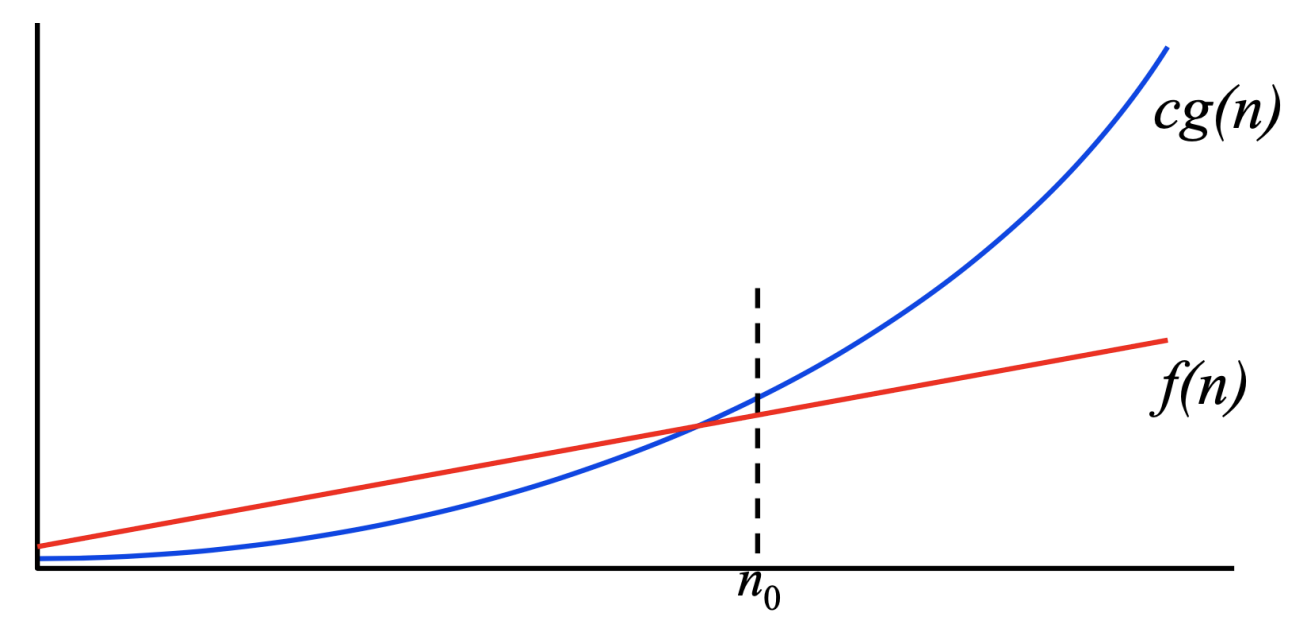
\includegraphics[width=6.5cm]{images/limite-superiore-asintotico-non-stretto.png}
	\vspace{-5pt}
	\caption{Limite superiore non stretto}
\end{wrapfigure}

\vspace{-15pt}
E immediato dalla definizione che:
\begin{center}
	$o(g(n)) \Longrightarrow O(g(n))$
\end{center}
Non vale il contrario: 
\begin{center}
	$2n^2 \in O(n^2) \land 2n^2 \notin o(n^2)$
\end{center}
Definizione alternativa:
\begin{center}
	$f(n) \in o(g(n)) \Longleftrightarrow \lim\limits_{n\to \infty}\frac{g(n)}{f(n)} = \infty$
\end{center}

\subsubsection{Limite inferiore asintotico non stretto}
\begin{definition}[Limite inferiore asintotico non stretto]
	Il limite inferiore asintotico non stretto si definisce come:
	\begin{center}
		$\omega(g(n)) = \{f(n) \mid \forall c \: \exists n_0 > 0 . \forall n > n_0, 0 \leq c \cdot g(n) \leq f(n) \}$
	\end{center}
\end{definition}
\noindent Si scrive come $f(n) \in \omega(g(n))$ oppure $f(n) = \omega(g(n))$ e si legge $f(n)$ è nell'ordine $\omega$ piccolo di $g(n)$.\\
$f(n)$ è limitata inferiormente da $g(n)$, ma non la raggiunge mai.\\
\begin{wrapfigure}[7]{l}{7cm}
	\vspace{-15pt}
	\centering
	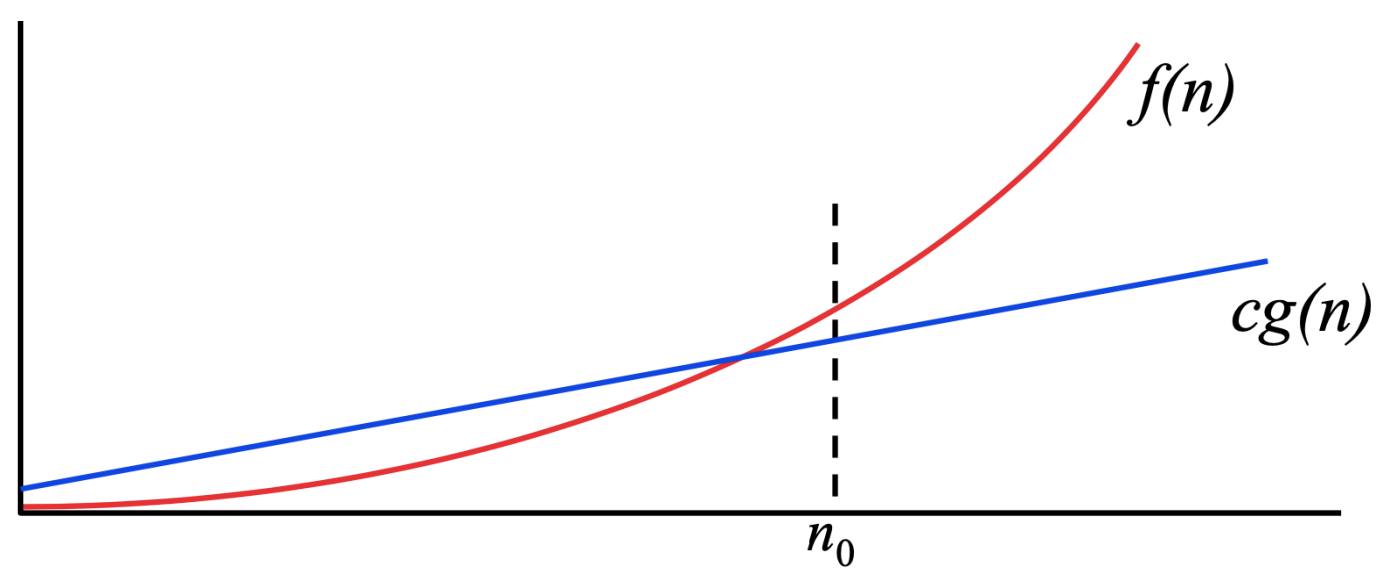
\includegraphics[width=6.5cm]{images/limite-inferiore-asintotico-non-stretto.png}
	\vspace{-5pt}
	\caption{Limite asintotico stretto}
\end{wrapfigure}

\vspace{-15pt}
E immediato dalla definizione che:
\begin{center}
	$\omega(g(n)) \Longrightarrow \Omega(g(n))$
\end{center}
Non vale il viceversa: 
\begin{center}
	$\frac{1}{5}n^2 \in \Omega(n^2) \land \frac{1}{2}n^2 \notin \omega(n^2)$
\end{center}
Definizione alternativa:
\begin{center}
	$f(n) \in \omega(g(n)) \Longleftrightarrow \lim\limits_{n\to \infty}\frac{g(n)}{f(n)} = 0$
\end{center}

\subsection{Equazioni di ricorrenza}
Quando un algoritmo contiene una chiamata \emph{ricorsiva} a se stesso, il suo tempo di esecuzione può essere descritto da una \textbf{equazione di ricorrenza}.
\begin{definition}[Ricorrenza]
	Una ricorrenza è un'equazione o una disequazione che descrive una funzione in termini del suo valore su input sempre più piccoli. \\
	Un'\textbf{equazione ricorsiva} esprime il valore di $T(n)$ come combinazione di $T(n_1), \ldots, T(n_h)$ dove $n_i < n, i=1,\ldots,h$:
	\begin{equation}
		T(n)=\begin{cases}
			c & n \leq k \\
			D(n) + \sum\limits_{i=1}^{h} T(n_i)+C(n) & n > k
		\end{cases}
	\end{equation}
\end{definition}
In un'equazione di ricorrenza:
\begin{itemize}
	\item $\mathbf{T(n)}$ è il \emph{tempo di esecuzione} di un problema di dimensione $n$
	\item Suddividiamo un problema in $a$ \textbf{sotto problemi}, ciascuno di dimensione $n/b$:
	\begin{itemize}
		\item $\mathbf{D(n)}$ è il tempo impiegato per \emph{suddividere} 
		\item $\mathbf{C(n)}$ per \emph{combinare} le soluzioni
	\end{itemize}
\end{itemize}
\begin{equation}
	T(n)=\begin{cases}
		\Theta(1) & n \leq k \\
		a \cdot T(\frac{n}{b}) + D(n) + C(n)) & n >k
	\end{cases}
\end{equation}
Alcuni casi particolari di equazioni ricorrenza sono quelle di \textbf{ordine k}:
\begin{equation}
	T(n)=\begin{cases}
		\Theta(1) & n \leq k \\
		\alpha_1 \cdot T(n-1) + \ldots + \alpha_k \cdot T(n-k) + f(n) & n >k
	\end{cases}
\end{equation}
e quelle \textbf{bilanciate}:
\begin{equation}
	T(n)=\begin{cases}
		\Theta(1) & n \leq k \\
		a \cdot T(\frac{n}{b}) + f(n) & n >k
	\end{cases}
\end{equation}
con $a \geq 1$, $b > 1$, $f$ asintoticamente positiva.

\subsubsection{Metodo iterativo}
Prendiamo come esempio l'algoritmo di ordinamento \emph{merge sort} e analizziamone la complessità:
\begin{lstlisting}[language=C, caption=Algoritmo merge sort, mathescape=true]
	void sort(int a[], size_t inizio, size_t fine, char order) {
		if ((fine - inizio) >= 1) {
			size_t centro1 = (inizio + fine)/2; $\Theta(1)$
			zie_t centro2 = centro1 + 1; $\Theta(1)$
			
			sort(a, inizio, centro1, order); T()
			sort(a, centro2, fine, order);
			
			merge(a, inizio, centro1, centro2, fine, order);
		}
	}
\end{lstlisting}
Ora scriviamo l'equazione di ricorrenza come segue:
\begin{equation}
	T(n)=\begin{cases}
		\Theta(1) & n \leq 1 \\
		2 \cdot T(\frac{n}{2}) + \Theta(n)) & n \geq 2
	\end{cases}
\end{equation}
Possiamo risolverla utilizzando il metodo iterativo, sapendo che dovremo fare $i = \log_2{n}$ iterazioni:

\begin{equation}
	\begin{split}
		T(n) = 2 \cdot T(\frac{n}{2})+c\cdot n = 2 \cdot (2 \cdot T(\frac{n}{4})+c\cdot \frac{n}{2}) +  c\cdot n = \\
		= 4 \cdot T(\frac{n}{4}) + c \cdot n + c \cdot n = 4 \cdot (2 \cdot T(\frac{n}{8}) + c \cdot \frac{n}{4}) + 2 \cdot c \cdot n = \\
		= 8 \cdot T(\frac{n}{8}) + c \cdot n + 2 \cdot c \cdot n = 8 \cdot T(\frac{n}{8}) + 3 \cdot c \cdot n = \\
		= \ldots = 2^i \cdot T(\frac{n}{2^i}) + i \cdot c \cdot n = 2^{\log_2{n}} \cdot T(1) + \log_2{n} \cdot c \cdot n = \\
		= n \cdot \Theta(1) + c \cdot n \cdot \log{n} = \Theta(n \cdot \log{n})
	\end{split}
\end{equation}
\subsubsection{Albero di ricorsione}
%TODO Inserire immagine per albero di ricorsione
\subsubsection{Master's Theorem}
Quando si tratta di risolvere equazioni di ricorrenza \textbf{bilanciate}, è possibile utilizzare il Master's Theorem. \\
\begin{equation}
	T(n)=\begin{cases}
		\Theta(1) & n \leq k \\
		a \cdot T(\frac{n}{b}) + f(n) & n >k
	\end{cases}
\end{equation}
L'intuizione consiste nel fare un confronto tra $f(n)$ e $n^{\log_b{a}}$, ovvero quante volte viene eseguito il passo ricorsivo. \\
Ci sono tre casi possibili:
\begin{itemize}
	\item \textbf{Minore}: $f(n) = O(n^{\log_b{a}-\epsilon})$ per qualche costante $\epsilon > 0$. \\ $f(n)$ cresce \textbf{polinomialmente} più lentamente di $n^{\log_b{a}}$ di un fattore $n^\epsilon$. \\
	\emph{Soluzione}: $T(n) = \Theta(n^{\log_b{a}})$ \\
	\begin{example}
		Data la seguente equazione di ricorrenza:
		\begin{equation}
			T(n) = 9 \cdot T(\frac{n}{3}) + n
		\end{equation}
		Abbiamo che $a=9$, $b=3$, $f(n) = n$, $n^{\log_3 9} = n^2$. Possiamo dedurre quindi che, per un $\epsilon = 1$:
		\begin{equation}
			f(n)  = n = O(n^{\log_3 9 - \epsilon}) = O(n)
		\end{equation}
	\end{example}
	\item \textbf{Uguale}: $f(n) = \Theta(n^{\log_b{a}}\cdot \ln^k{n})$ per qualche costante $k \geq 0$. \\ $f(n)$ e $n^{\log_b{a}}$ crescono allo stesso modo. \\
	\emph{Soluzione}: $T(n) = \Theta(n^{\log_b{a}} \cdot \ln^{k+1}{n})$
	\item \textbf{Maggiore}: $f(n) = \Omega(n^{\log_b{a} + \epsilon})$ per qualche costante $\epsilon > 0$. \\ $f(n)$ cresce \textbf{polinomialmente} più in fretta di $n^{\log_b{a}}$ di un fattore $N^\epsilon$ e rispetta la \textbf{condizione di regolarità}: $a \cdot f(\frac{n}{b}) \leq c \cdot f(n)$ per qualche costante $c<1$ e $n > n_0$. \\
	\emph{Soluzione}: $T(n) = \Theta(f(n))$
\end{itemize}
\begin{observation}
	Il Master's Theorem si può usare solamente quando $f(x)$ cresce \textbf{polinomialmente} più in fretta o lentamente di $n^{\log_b{a}}$. Ad esempio se avessimo $f(x) = \log{n}$ non potremmo utilizzarlo.
\end{observation}